\section{Stereo PIV Data processing}

Raw PIV data was processed into text files containing lists of vectors and 
positions from raw image data with commercial INSIGHT software. 
This format is considered to be the 
starting point for the present analysis. Each vector is recorded as a row in a 
"v3d" file, with a set of position coordinates,velocity 
vector components, and two quality control flags that were used to reduce 
spurious vector count. An example of this data is shown in Table 
\ref{table:v3d_row_example}.

\begin{table}[H]
\begin{center}
\begin{tabular}{|cccccccc|}
	\hline
	X mm & Y mm  & Z mm & U m/s & V m/s & W m/s & CHC & Residual Pixels\\
	\hline
	8.02046 & 0.174553 & 0 & 0.415872 & -2.25951 & 13.5873 & 1 & 0.127058\\
	9.74656 & 0.174553 & 0 & 0.386507 & -2.4523 & 13.9244 & 1 & 0.166965\\
	11.4727 & 0.174553 & 0 & 1.01919 & -2.8773 & 14.9454 & 1 & 0.0480147\\
	13.1988 & 0.174553 & 0 & 1.30872 & -3.02836 & 15.2081 & 1 & 0.0560525\\
	\hline
\end{tabular}
\caption{Example rows from v3d files with raw 3d vector data}
\label{table:v3d_row_example}
\end{center}
\end{table}


The position coordinates are expressed in units of millimeters from 
the fiducial mark on the target used for calibration. These coordinates are 
expressed from the viewpoint of the cameras, which were pointed upstream; 
positive $X$ coordinates are to the right, positive $Y$ is upwards, and 
positive $Z$ is towards the cameras. Vector components are recorded as $U$, 
$V$ and $W$. 

\subsection{Reynolds Averaging}
Since each run contained 200 separate vector sets, this data needed to be 
synthesized into 
values that compare well with the Reynolds Averaged Navier Stokes equations in 
cylindrical coordinates. This processing was performed in Python 2.7 and 
Matlab, with much of the code entirely replicated in each language. 
First, text files with tables of vector data were loaded into a parser to 
construct a mesh grid of the $X$, $Y$ coordinate space. These mesh grids 
establish the relationship between matrix indices and real coordinate 
space with units of $mm$.
Then, for each test as shown in Table \ref{table:test_matrix_table}, data from 
each of the 200 snapshots is Reynolds averaged to produce a stable velocity 
component, and a fluctuating velocity component in each dimension for each 
vector, as expressed in equation \ref{eq:rans_components} in terms of position 
$x$ at time $t$.

\begin{equation}
u(x,t) = \overline{u}(x) + u^\prime(x,t)
\label{eq:rans_components}
\end{equation}


Each component is given an individual variable name, with stable nonfluctuating 
components taken from a simple average of all sets expressed as the component 
letter with an over bar ($\overline{u}$, $\overline{v}$, $\overline{w}$), and 
time averaged fluctuating component expressed with a prime 
($\overline{u^\prime}$, $\overline{v^\prime}$, $\overline{w^\prime}$). 
Velocities referring to just one of the 200 sets will use a 
subscript $i$ as ($u_i$, $v_i$, $w_i$). The stable components are computed with 
a simple average to preserve the sign, while the fluctuating components are 
computed with a root mean squared method as shown in equations \ref{eq:ubar} 
through \ref{eq:wprime}.

\begin{equation}
\overline{u}  = \frac{1}{N} \sum_{i=1}^{200} u_i
\label{eq:ubar}
\end{equation}

\begin{equation}
\overline{v}  = \frac{1}{N} \sum_{i=1}^{200} v_i
\end{equation}

\begin{equation}
\overline{w}  = \frac{1}{N} \sum_{i=1}^{200} w_i
\end{equation}

\begin{equation}
\overline{u^\prime} = \sqrt{\frac{1}{N-1} \sum_{i=1}^{200} (u_i - 
\overline{u})^2}
\end{equation}

\begin{equation}
\overline{v^\prime} = \sqrt{\frac{1}{N-1} \sum_{i=1}^{200} (v_i - 
\overline{v})^2}
\end{equation}

\begin{equation}
\overline{w^\prime} = \sqrt{\frac{1}{N-1} \sum_{i=1}^{200} (w_i - 
\overline{w})^2}
\label{eq:wprime}
\end{equation}

Where $\overline{u}$, $\overline{v}$ and $\overline{w}$ are the time averaged 
velocity 
components in the $X$, $Y$, $Z$ directions respectively, and  
$\overline{u^\prime}$, $\overline{v^\prime}$ and $\overline{w^\prime}$ are the 
time averaged fluctuating velocity components.

Similarly, time averaged Reynolds stresses can be calculated by multiplying the 
fluctuating components together before taking the root mean square average by 
equations \ref{eq:rs_uu} through \ref{eq:rs_vw}.

\begin{equation}
\overline{u^\prime u^\prime} = \sqrt{\frac{1}{N-1} \sum_{i=1}^{200} 
	((u_i - \overline{u})(u_i - \overline{u}))^2}
\label{eq:rs_uu}
\end{equation}

\begin{equation}
\overline{v^\prime v^\prime} = \sqrt{\frac{1}{N-1} \sum_{i=1}^{200} 
	((v_i - \overline{v})(v_i - \overline{v}))^2}
\end{equation}

\begin{equation}
\overline{w^\prime w^\prime} = \sqrt{\frac{1}{N-1} \sum_{i=1}^{200} 
	((w_i - \overline{w})(w_i - \overline{w}))^2}
\end{equation}

\begin{equation}
\overline{u^\prime v^\prime} = \sqrt{\frac{1}{N-1} \sum_{i=1}^{200} 
	((u_i - \overline{u})(v_i - \overline{v}))^2}
\end{equation}

\begin{equation}
\overline{u^\prime w^\prime} = \sqrt{\frac{1}{N-1} \sum_{i=1}^{200} 
	((u_i - \overline{u})(w_i - \overline{w}))^2}
\end{equation}

\begin{equation}
\overline{v^\prime w^\prime} = \sqrt{\frac{1}{N-1} \sum_{i=1}^{200} 
	((v_i - \overline{v})(w_i - \overline{w}))^2}
\label{eq:rs_vw}
\end{equation}

Turbulent kinetic energy $k$ can be calculated as one half 
of the sum of the three double correlation components as in equation 
\ref{eq:tke}.

\begin{equation}
k = \frac{1}{2} \left(\overline{u^\prime u^\prime}^2 + 
	\overline{v^\prime v^\prime}^2 + 
	\overline{w^\prime w^\prime}^2\right)
\label{eq:tke}
\end{equation}


Once all the statistics for Cartesian coordinates have been generated, the 
vortex core must be found in order to convert all values to cylindrical 
coordinates. The core is found by finding the minimum in-plane velocity 
magnitudes near the center of the interrogation plane, excluding the stream 
wise $w$ component. In practice, to avoid confusion in identifying the vortex 
core due to spurious edge values, a threshold value is defined that limits the 
search for in-plane velocity minima to an area near the center of the field of 
view. Once the lowest value was found, sub-grid accuracy was 
achieved by taking a cubic interpolation of the grid points surrounding the 
minimum. This technique was sufficiently robust to automatically identify the 
core correctly in every test.

With a location for the vortex core, new mesh grids in radial and tangential 
coordinates, $R$ and $\theta$, are created from the $X$ and 
$Y$ mesh grids. Velocity components, $r$ and $t$,are then 
calculated by equations \ref{eq:uv_r} and \ref{eq:uv_t}.

\begin{equation}
r_i = u_i \cos{(\theta)} + v_i \sin{(\theta)}
\label{eq:uv_r}
\end{equation}

\begin{equation}
t_i = u_i \sin{(\theta)} - v_i \cos{(\theta)}
\label{eq:uv_t}
\end{equation}

Where $r_i$ and $t_i$ represent a radial and tangential velocity matrix for 
just one of the 200 total surveys, and $\theta$ is the mesh grid of angles 
about the vortex core. These equations were applied on an element wise basis to 
every grid point in the vector field. Once this was done, the same Reynolds 
averaging technique was applied to separate the radial and tangential velocity 
components $r$ and $t$ into stable and fluctuating components in equations 
\ref{eq:rbar} through \ref{eq:tprime}.

\begin{equation}
\overline{r}  = \frac{1}{N} \sum_{i=1}^{200} r_i
\label{eq:rbar}
\end{equation}

\begin{equation}
\overline{t}  = \frac{1}{N} \sum_{i=1}^{200} t_i
\label{eq:tbar}
\end{equation}

\begin{equation}
\overline{r^\prime} = \sqrt{\frac{1}{N-1} \sum_{i=1}^{200} (r_i - 
\overline{r})^2}
\label{eq:rprime}
\end{equation}

\begin{equation}
\overline{t^\prime} = \sqrt{\frac{1}{N-1} \sum_{i=1}^{200} (t_i - 
\overline{t})^2}
\label{eq:tprime}
\end{equation}

The double correlations in cylindrical coordinates were calculated directly 
from the transformed cylindrical velocities with equations \ref{eq:rs_rr) 
through \ref{eq:rs_tw}.
	
\begin{equation}
\overline{r^\prime r^\prime} = \sqrt{\frac{1}{N-1} \sum_{i=1}^{200} 
	((r_i - \overline{r})(r_i - \overline{r}))^2}
\label{eq:rs_rr}
\end{equation}

\begin{equation}
\overline{t^\prime t^\prime} = \sqrt{\frac{1}{N-1} \sum_{i=1}^{200} 
	((t_i - \overline{t})(t_i - \overline{t}))^2}
\end{equation}

\begin{equation}
\overline{r^\prime t^\prime} = \sqrt{\frac{1}{N-1} \sum_{i=1}^{200} 
	((r_i - \overline{r})(t_i - \overline{t}))^2}
\end{equation}

\begin{equation}
\overline{r^\prime w^\prime} = \sqrt{\frac{1}{N-1} \sum_{i=1}^{200} 
	((r_i - \overline{r})(w_i - \overline{w}))^2}
\end{equation}

\begin{equation}
\overline{t^\prime w^\prime} = \sqrt{\frac{1}{N-1} \sum_{i=1}^{200} 
	((t_i - \overline{t})(w_i - \overline{w}))^2}
\label{eq:rs_tw}
\end{equation}

	
Once this processing is complete, we have large set of Reynolds averaged 
velocity data available for each of the 70 test cases. Plots of this data from 
test case 55 will be shown as examples. Stream plots can be produced as in 
figure \ref{fig:examp_stream}. Cartesian average velocity components for test 
case is shown in figures \ref{fig:examp_U} through \ref{fig:examp_W}, though 
they are not particularly useful when compared to values in cylindrical 
coordinates. 
Cylindrical average velocity components are shown in figures \ref{fig:examp_R} 
and \ref{fig:examp_T}. Reynolds stresses are shown in figures 
\ref{fig:examp_rt} through \ref{fig:examp_tw}. Turbulent energies are shown in 
figures \ref{fig:examp_rr} through \ref{fig:examp_ww}. Total turbulent kinetic 
energy $k$ is shown in figure \ref{fig:examp_tke}. Scatter plots that 
flatten the dataset into one dimension can be generated as in the tangential 
velocity vs distance to core plot shown in figure \ref{fig:examp_Tscatter}. 

\begin{figure}[H]
	\centering
	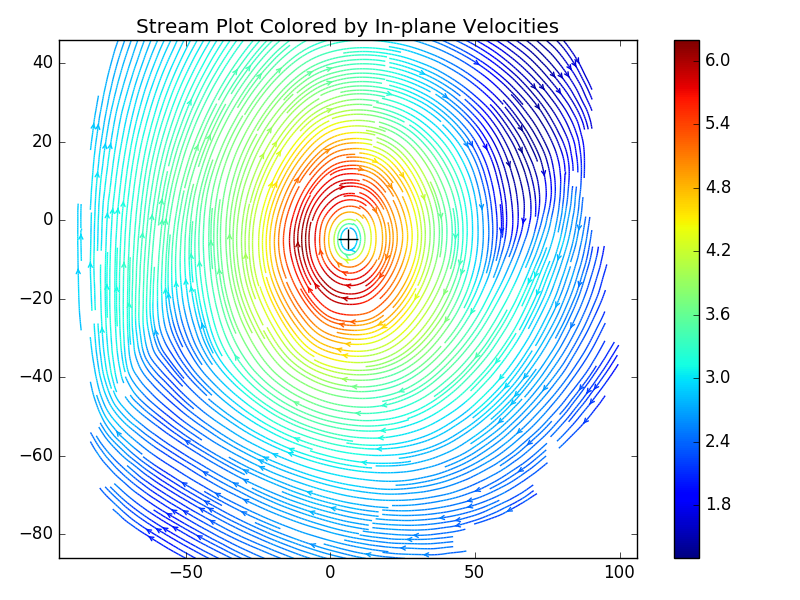
\includegraphics[width=5in]{figs/example_vortex_figs/example_stream}
	\caption{Example stream plot.}
	\label{fig:examp_stream}
\end{figure}

\begin{figure}[H]
	\centering
	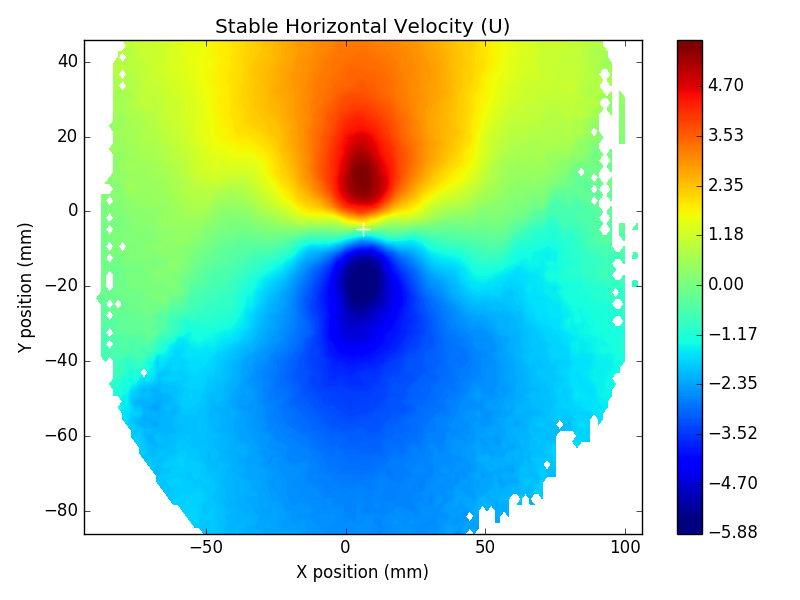
\includegraphics[width=5in]{figs/example_vortex_figs/example_U_contour}
\caption{Example contour plot of $\overline{u}$.}
\label{fig:examp_U}
\end{figure}

\begin{figure}[H]
	\centering
	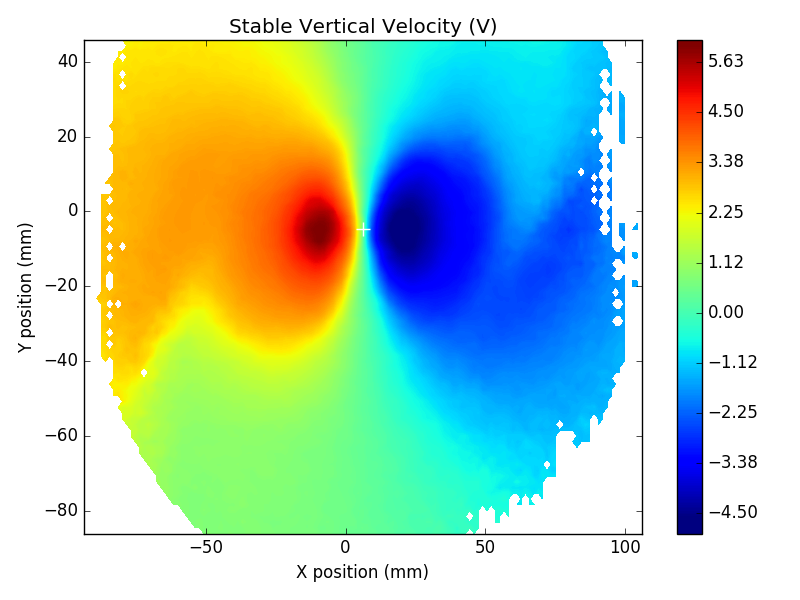
\includegraphics[width=5in]{figs/example_vortex_figs/example_V_contour}
\caption{Example contour plot of $\overline{v}$.}
\label{fig:examp_V}
\end{figure}

\begin{figure}[H]
	\centering
	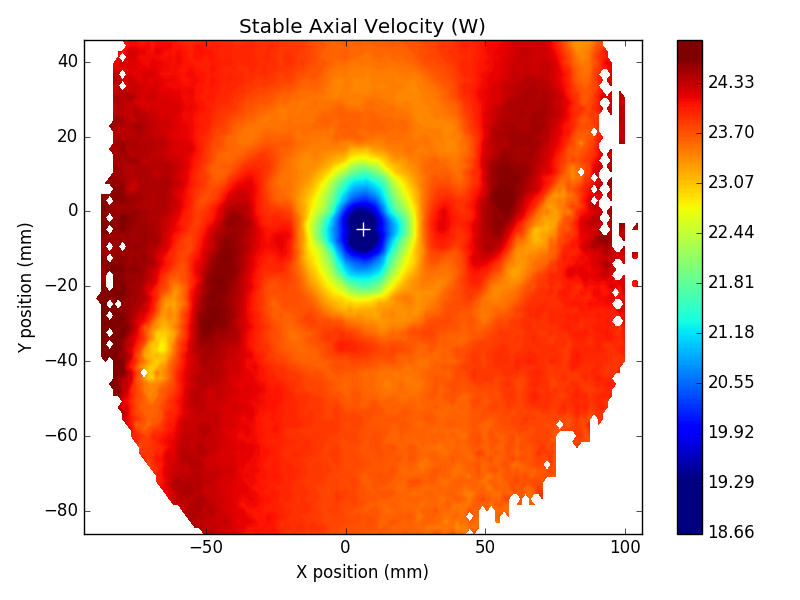
\includegraphics[width=5in]{figs/example_vortex_figs/example_W_contour}
\caption{Example contour plot of $\overline{w}$.}
\label{fig:examp_W}
\end{figure}

\begin{figure}[H]
	\centering
	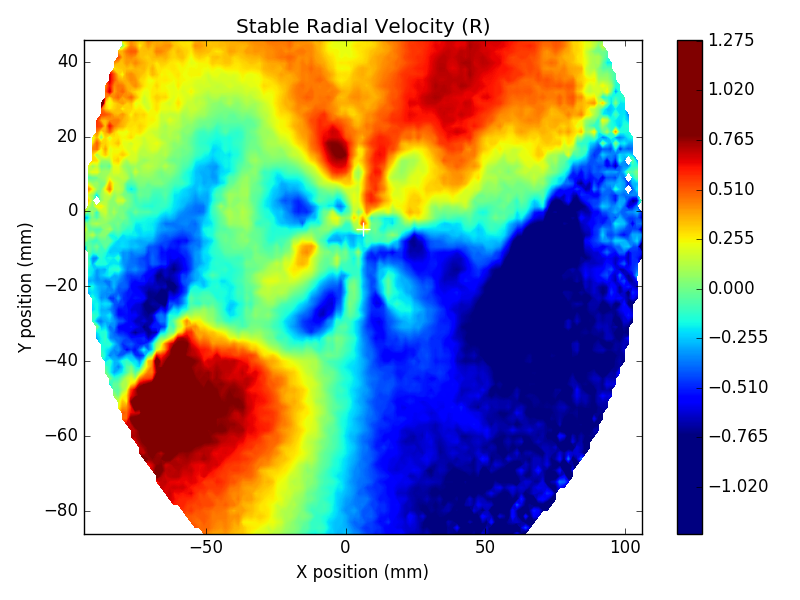
\includegraphics[width=5in]{figs/example_vortex_figs/example_R_contour}
\caption{Example contour plot of $\overline{r}$.}
\label{fig:examp_R}
\end{figure}

\begin{figure}[H]
	\centering
	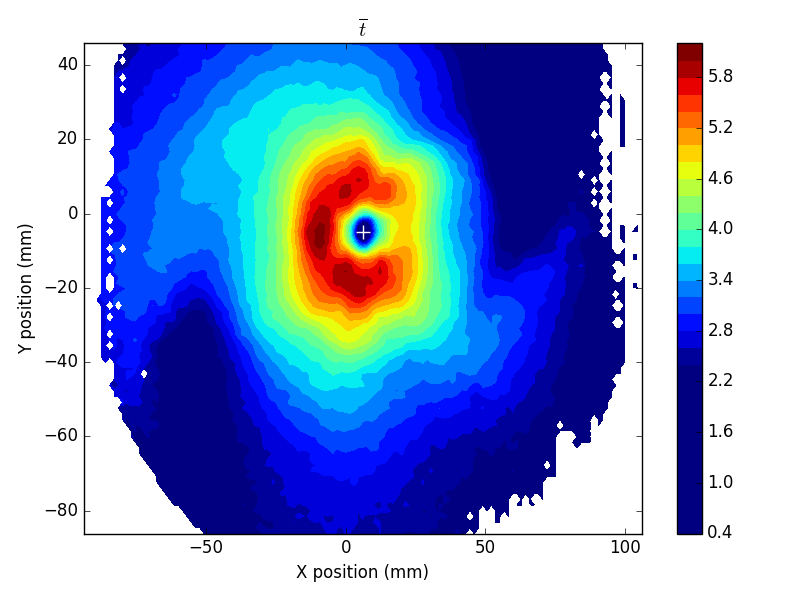
\includegraphics[width=5in]{figs/example_vortex_figs/example_T_contour}
\caption{Example contour plot of $\overline{t}$.}
\label{fig:examp_T}
\end{figure}

\begin{figure}[H]
	\centering
	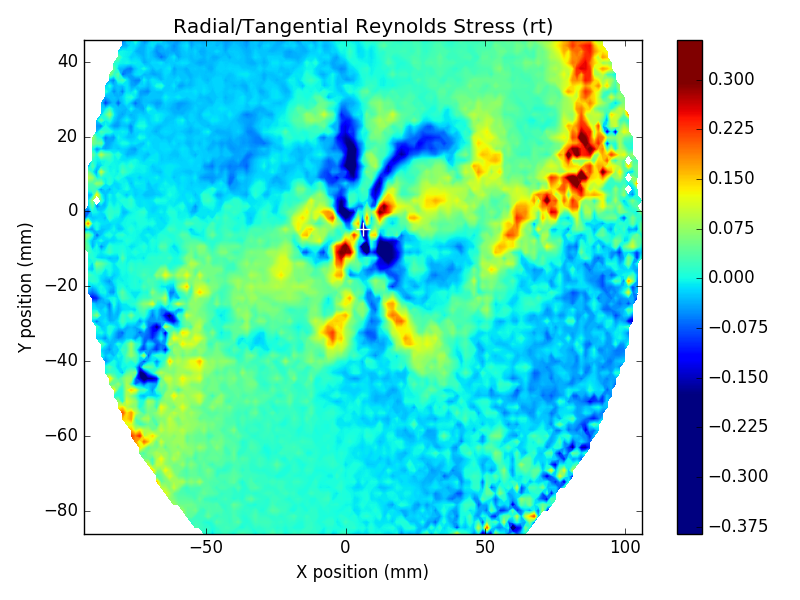
\includegraphics[width=5in]{figs/example_vortex_figs/example_rt_contour}
\caption{Example contour plot of $\overline{r^\prime t^\prime}$.}
\label{fig:examp_rt}
\end{figure}

\begin{figure}[H]
	\centering
	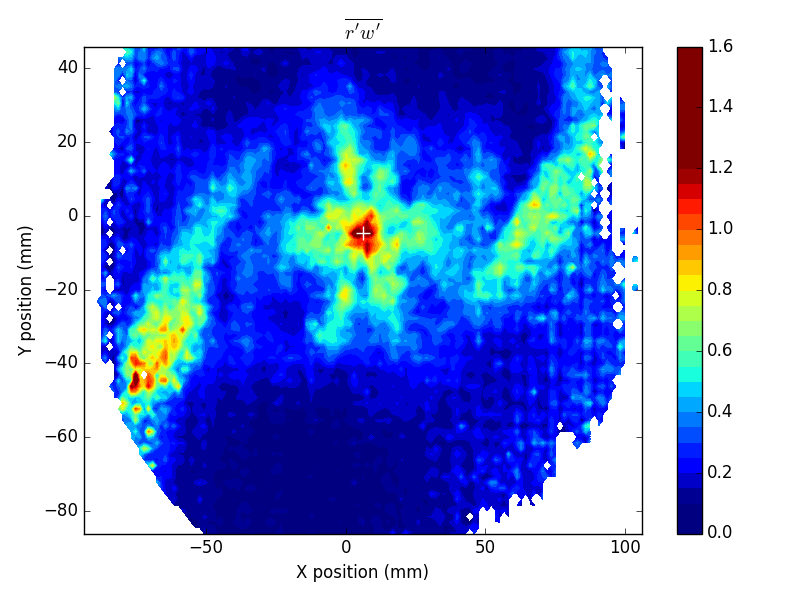
\includegraphics[width=5in]{figs/example_vortex_figs/example_rw_contour}
\caption{Example contour plot of $\overline{r^\prime w^\prime}$.}
\label{fig:examp_rw}
\end{figure}

\begin{figure}[H]
	\centering
	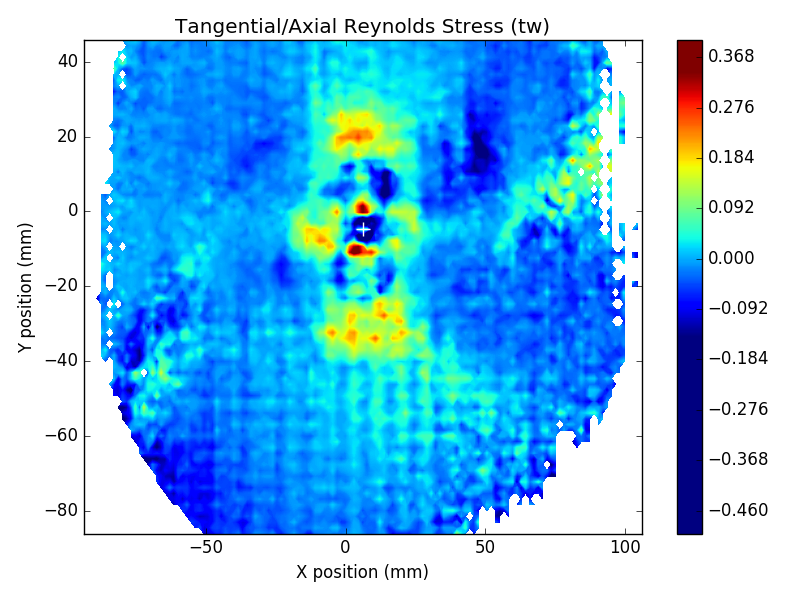
\includegraphics[width=5in]{figs/example_vortex_figs/example_tw_contour}
\caption{Example contour plot of $\overline{t^\prime w^\prime}$.}
\label{fig:examp_tw}
\end{figure}

\begin{figure}[H]
	\centering
	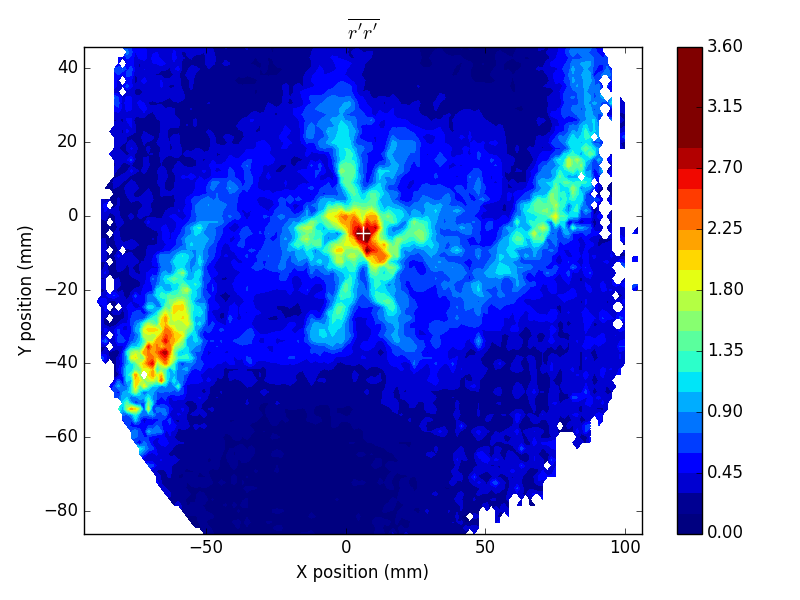
\includegraphics[width=5in]{figs/example_vortex_figs/example_rr_contour}
\caption{Example contour plot of $\overline{r^\prime r^\prime}$.}
\label{fig:examp_rr}
\end{figure}

\begin{figure}[H]
	\centering
	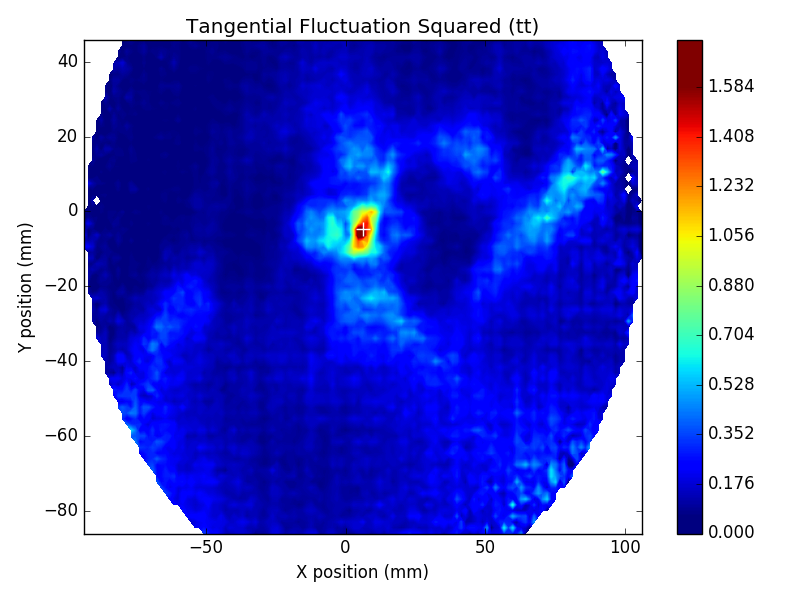
\includegraphics[width=5in]{figs/example_vortex_figs/example_tt_contour}
\caption{Example contour plot of $\overline{t^\prime t^\prime}$.}
\label{fig:examp_tt}
\end{figure}

\begin{figure}[H]
	\centering
	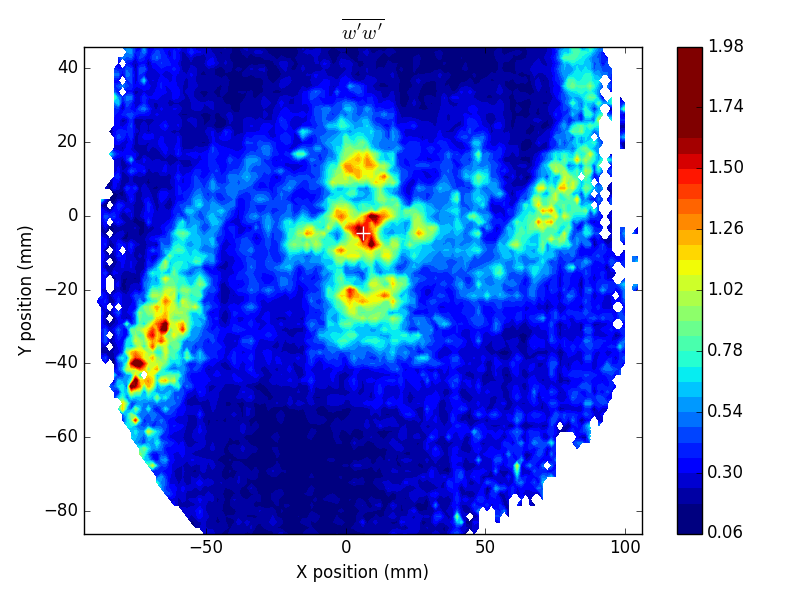
\includegraphics[width=5in]{figs/example_vortex_figs/example_ww_contour}
\caption{Example contour plot of $\overline{w^\prime w^\prime}$.}
\label{fig:examp_ww}
\end{figure}

\begin{figure}[H]
	\centering
	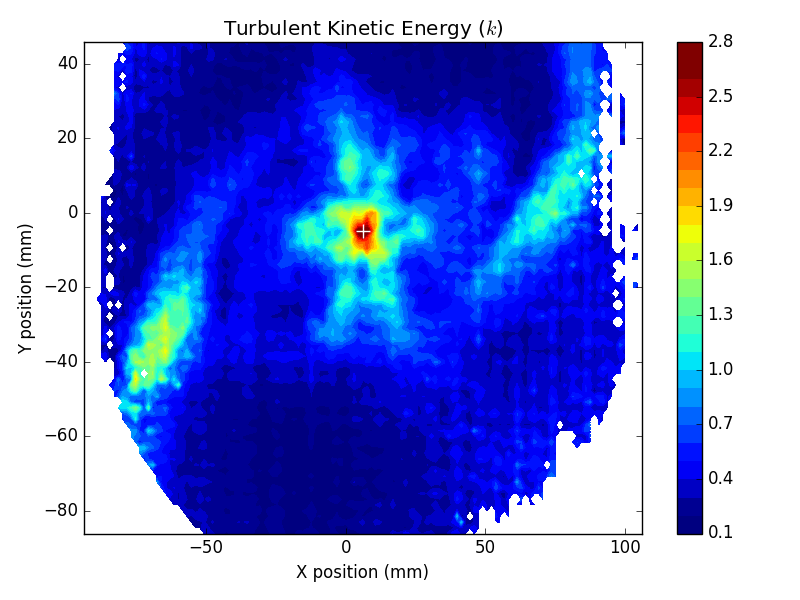
\includegraphics[width=5in]{figs/example_vortex_figs/example_ctke_contour}
\caption{Example contour plot of turbulent kinetic energy $k$.}
\label{fig:examp_tke}
\end{figure}

\begin{figure}[H]
	\centering
	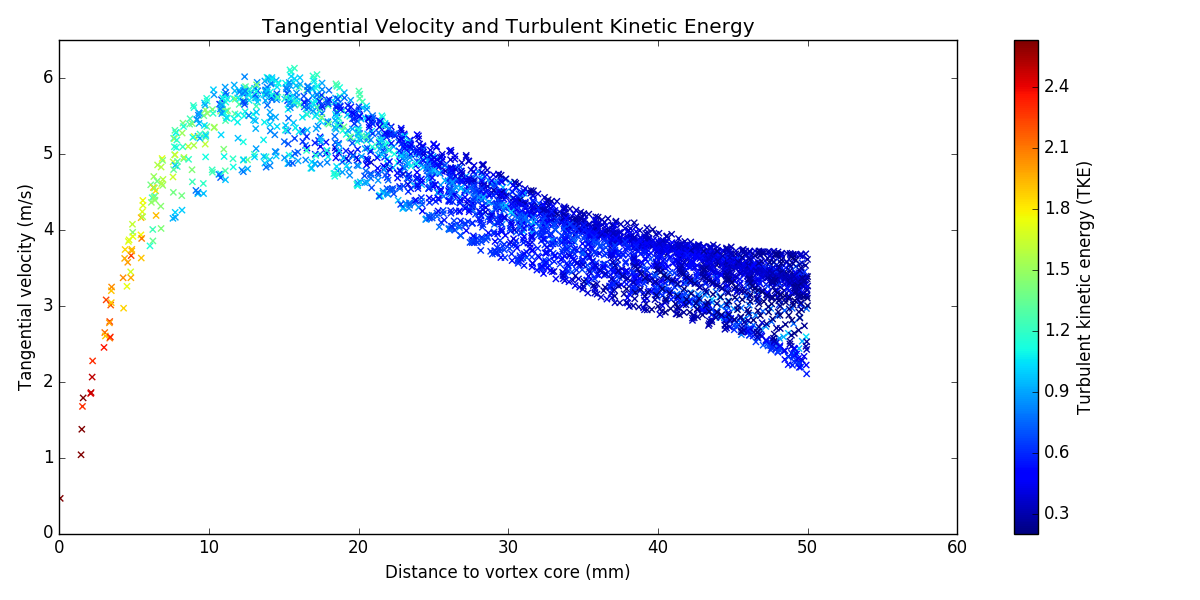
\includegraphics[width=7in]{figs/example_vortex_figs/example_TscatterTKE}
\caption{Example scatter plot of $T$, colored by $k$.}
\label{fig:examp_Tscatter}
\end{figure}

Insight to the quality and uncertainty in each measurement was gained by 
examining the number of vectors successfully extracted from the set of 200 
snapshots as shown in Figure \ref{fig:example_num_contour}. Locations with 
fewer than twenty valid vectors in the set of 200 were thrown out. A clear 
relationship between the total turbulent kinetic energy, $k$, and the number of 
vectors making up the average was observed, and is discussed in Chapter 3.

\begin{figure}[H]
	\centering
	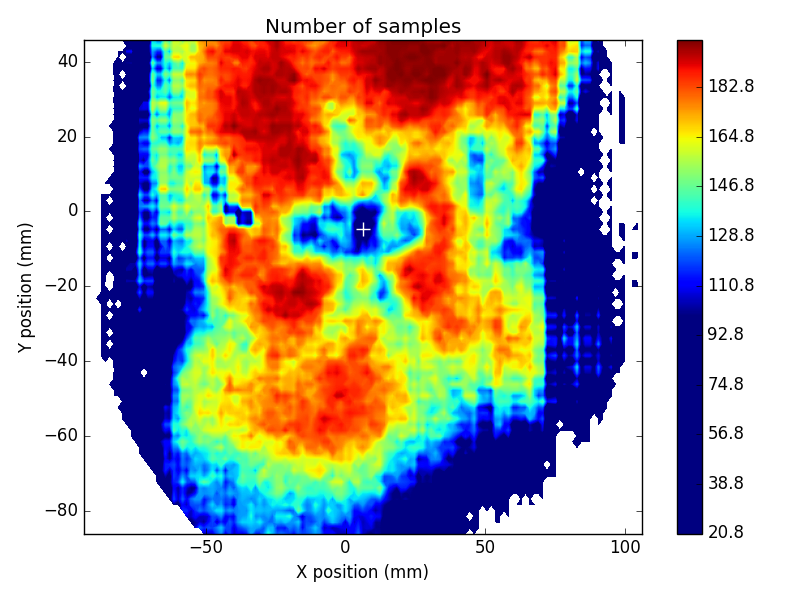
\includegraphics[width=5in]{figs/example_vortex_figs/example_num_contour}
	\caption{Example contour plot showing the variation in the number of 
	measurements within the interrogation plane}
	\label{fig:example_num_contour}
\end{figure}
